\section{Task Visualizations}
\label{sec:task_visualizations}

\subsection{HumanoidArena Tasks}
\label{sec:vis_humanoidarena}

\begin{figure}[H]
  \centering
  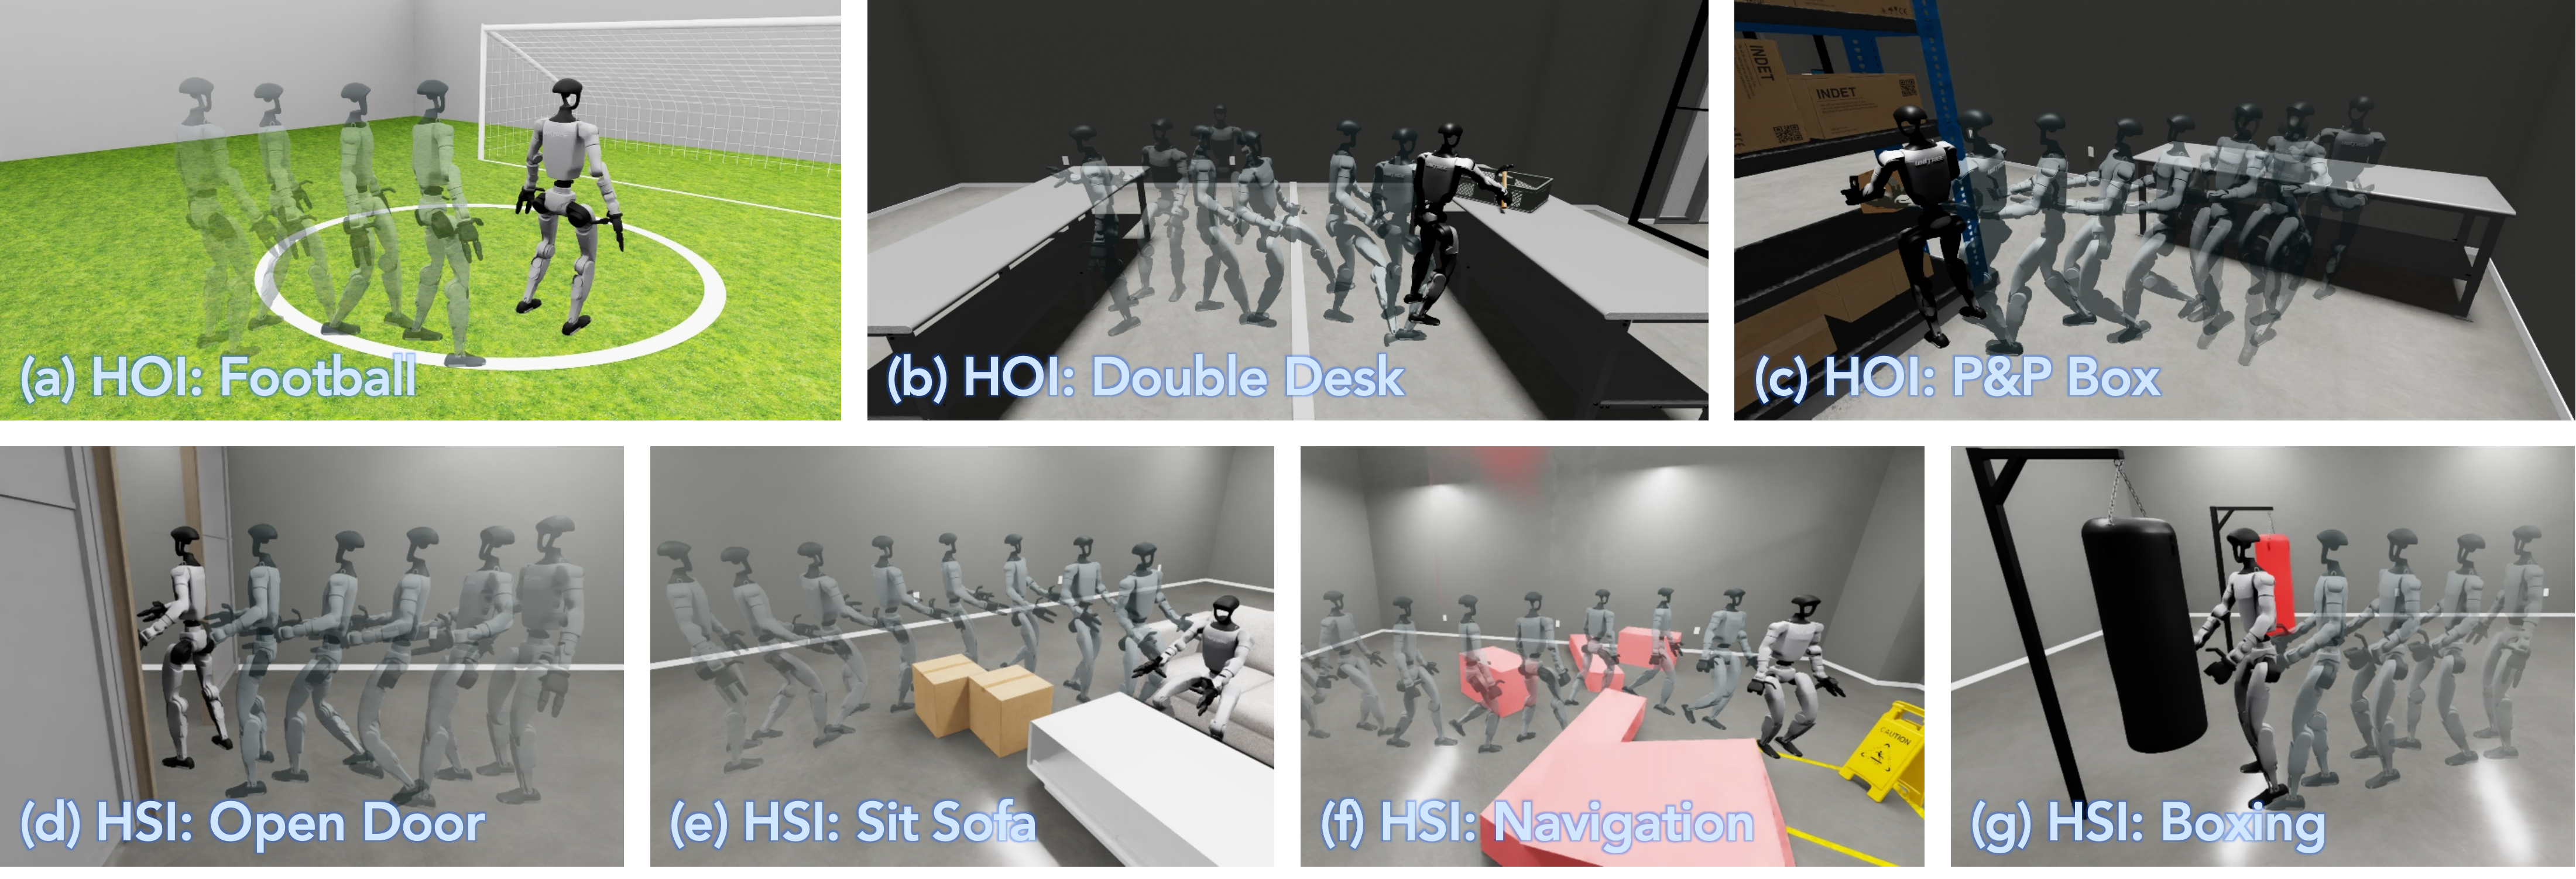
\includegraphics[width=\textwidth]{image/arena.png}
  \caption{\textbf{Visualization of the Seven HumanoidArena Tasks.} The benchmark includes Football, DoubleDesk, P\&Pbox, OpenDoor, SitSofa, Boxing, and VisNavi, covering language-conditioned humanoid behavior across human--object and human--scene interaction with coordinated locomotion, balance, and manipulation.}
  \label{fig:humanoidarena}
\end{figure}

\subsection{SIMPLE Tasks}
\label{sec:vis_simple}

\begin{figure}[H]
  \centering
  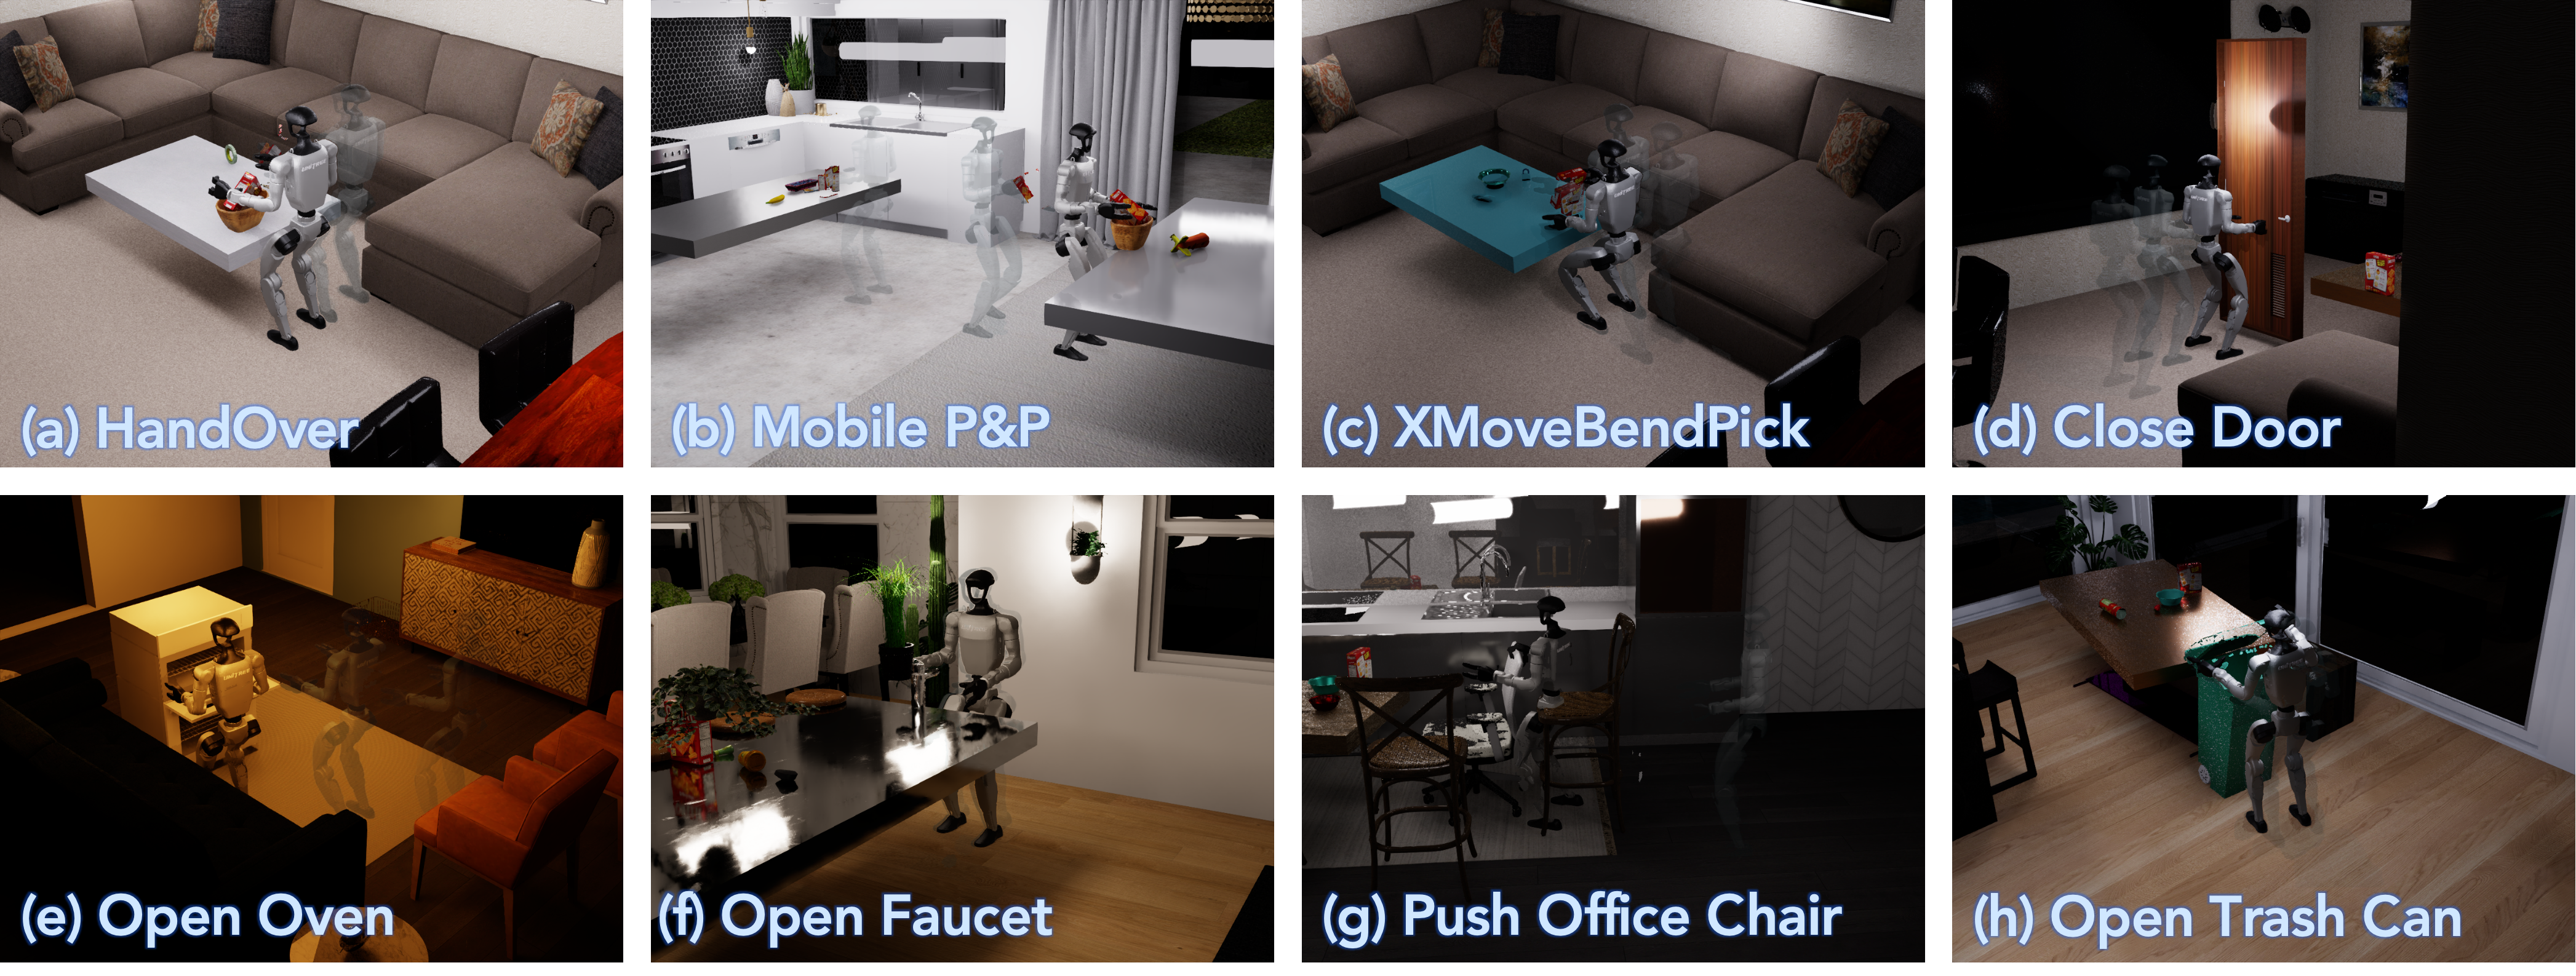
\includegraphics[width=\textwidth]{image/simple.png}
  \caption{\textbf{Evaluated SIMPLE Task Suite.} The selected tasks cover object handover and mobile pick-and-place, locomotion-integrated object pickup, articulated-object interaction, and household-object manipulation. Panels show (a) Handover, (b) Mobile P\&P, (c) XMoveBendPick, (d) CloseDoor, (e) OpenOven, (f) OpenFaucet, (g) Push Office Chair, and (h) OpenTrashCan.}
  \label{fig:simple_tasks}
\end{figure}

\clearpage
\subsection{Real-World Tasks}
\label{sec:vis_real_world}

\begin{figure}[H]
  \centering
  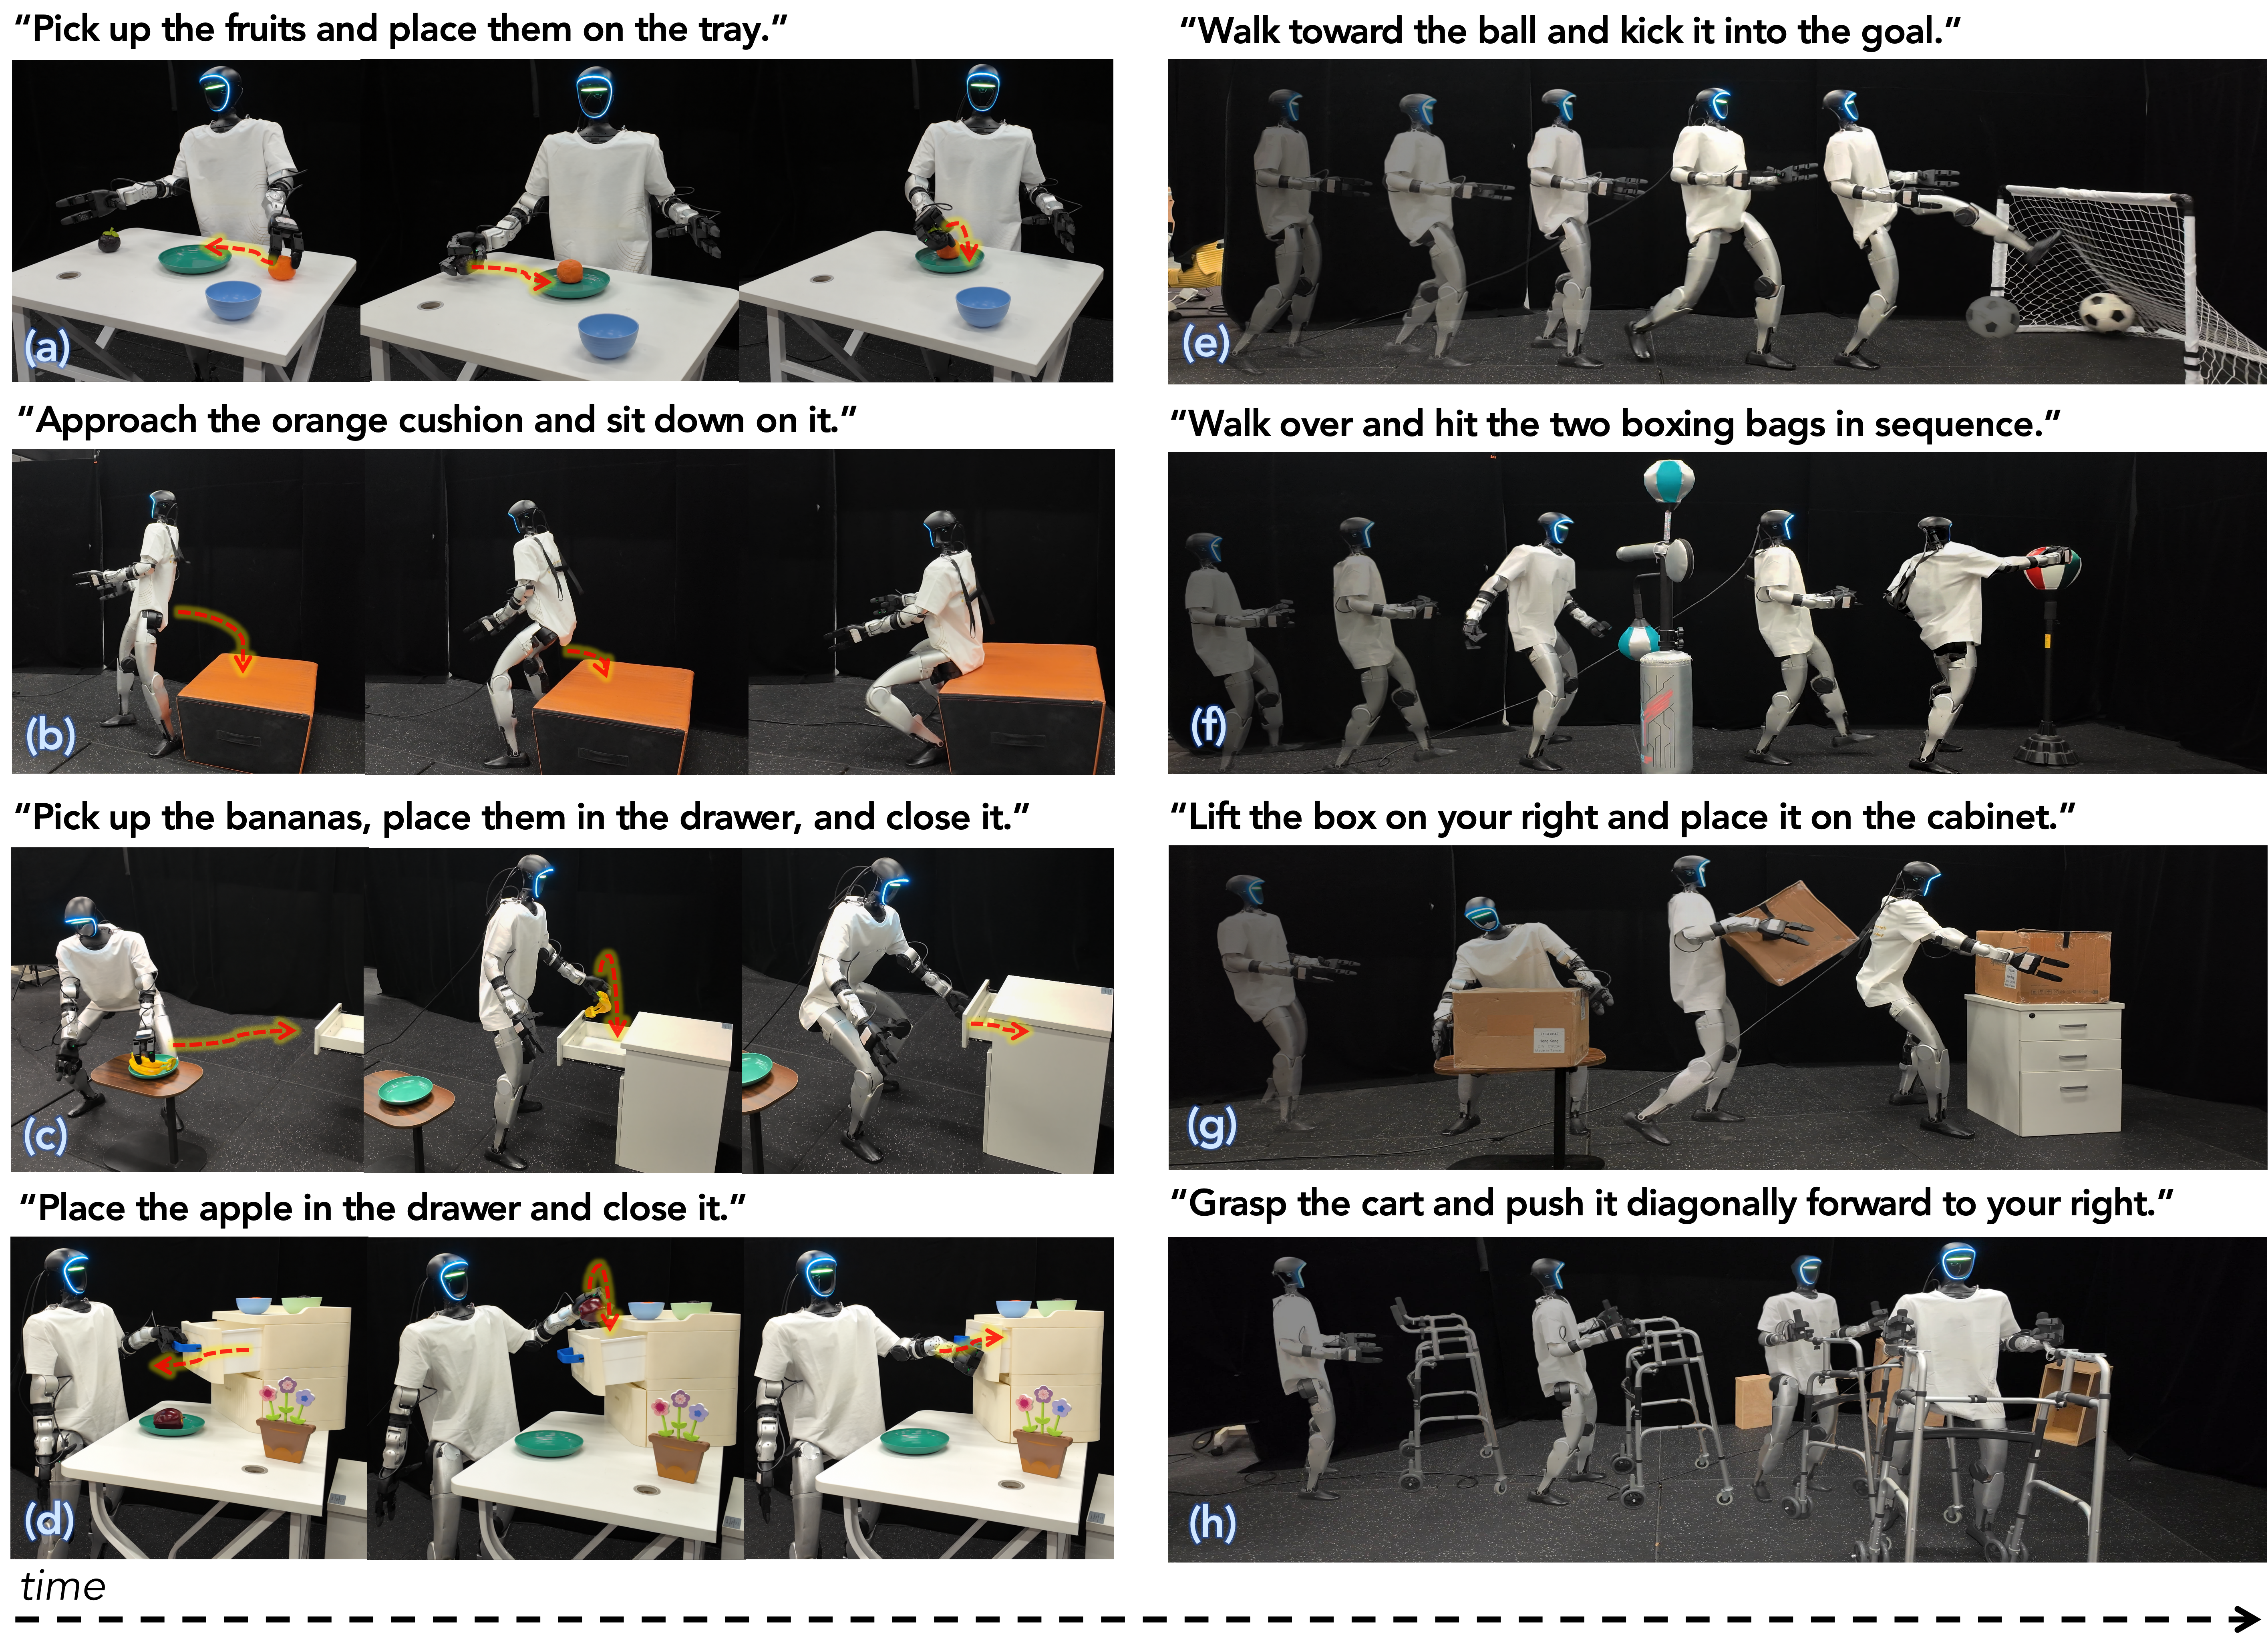
\includegraphics[width=\textwidth]{image/real_world.png}
  \caption{\textbf{Examples of Real-World Humanoid Manipulation.} The image shows representative interaction scenarios involving articulated objects, object transport, and coordinated whole-body motion.}
  \label{fig:real_world}
\end{figure}
